\begin{frame}{Sum up}
	\centering
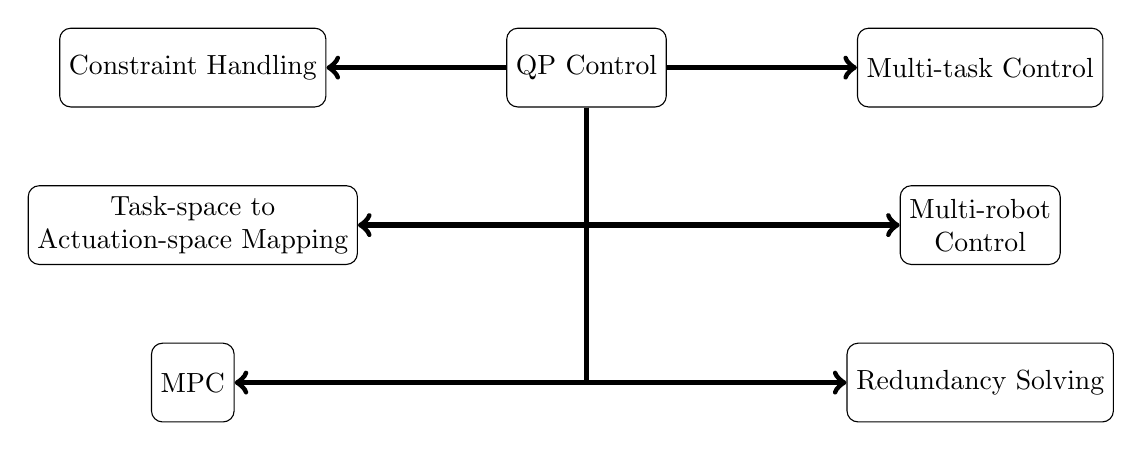
\begin{tikzpicture}[node distance=2cm]
	
	% Style for the boxes
	\tikzstyle{box}=[
	rectangle,
	draw,
	rounded corners,
%	minimum width=3.5cm,
	minimum height=1cm,
	align=center
	]
	%	\node [block] (CRA) at (-1, 12) {Complex robotic application};
		\node[box] (QP) at (-1, 0) {QP Control};
	% --- First row ---
	\node[box] (MTC) at (4, 0)  {Multi-task Control};
	
	\node[box] (CH) at (-6, 0){Constraint Handling};
	
	% --- Second row ---
	\node[box] (MRC) at (4, -2) {Multi-robot\\ Control};
	\node[box] (MPC) at (-6, -4) {MPC};
	\node[box] (RS) at (4, -4) {Redundancy Solving};
	\node[box] (TS2AS) at (-6, -2) {Task-space  to\\ Actuation-space Mapping};
	\draw[->,line width=2pt] (QP) -- (CH);
	\draw[->,line width=2pt] (QP) -- (MTC);
	\draw[->,line width=2pt] (QP) |- (TS2AS);
	\draw[->,line width=2pt] (QP) |- (MRC);
	\draw[->,line width=2pt] (QP) |- (MPC);
	\draw[->,line width=2pt] (QP) |- (RS);
\end{tikzpicture}

\end{frame}

\begin{frame}{QP Limitations}
%	The current limitations are related to different aspects
	\begin{itemize}
		\item Model based: accurate robot model is required
		\item  Not straightforward extendable to non-control-affine systems
		\item No analytical solution $\Rightarrow$ Scepticism about stability certification... 
		\item QP is myopic (\emph{cannot see beyond the current time}): 
		getting stuck in undesired local minima eventhough a feasible solution exists		
		\item No guarantees for the existance of a feasile solution  during the runtime %Mitigating constraints conflict/incompatibility
		\item Tasks priority (weights or lexicographic order) and gains tuning (tuning again!)				
		\item Scalability to high-DoF robots (multi-robot QP)
	%	\item On-the-fly incerting of constraints: QP compatibilty and numerical discontinuities
		\item Difficulty in debugging the ‘QP fail’!
	\end{itemize}
\end{frame}
\begin{frame}{Further research}
	\begin{itemize}
		\item How to render QP conflict-aware? Constraints may arise for multiple reasons, add prediction + work on the task targets	 
		\item Whole-body MPC with explicit constraints handling
		\item Task priority adaptation
		\item Tasks scheduling
		\item Multi-robot control: centralized vs distributed control, hierarchical MPC
		\item Integration with learning: reinforcement learning layer on top of whole-body QP  
		\item Efficient QP solvers: reduce computation time by exploiting matrices' sparity
		\end{itemize}
\end{frame}
\begin{frame}{Embodiment - Robots as embodied avatars}
		\begin{picture}(0,0)
%		\put(0,70){Robots are able to accomplish complex missions...}
		\put(70,-20){\begin{minipage}{0.7\columnwidth}
				\centering
				\embedvideo*{\includegraphics[width=\columnwidth]{Screenshot from 2025-11-14 18-07-00.png}}{Figures/embodiment_avatar.mp4}[autoplay=false,showGUI=true]\\
				\makebox{\hspace{0cm}\centering\small Sci-fi in the Avatar movie (2009)}
		\end{minipage}}
	\end{picture}
\end{frame}
\begin{frame}{Embodiment - Robots as embodied avatars}
	\begin{picture}(0,0)
		%		\put(0,70){Robots are able to accomplish complex missions...}
		\put(70,-20){\begin{minipage}{0.7\columnwidth}
				\centering
				\embedvideo*{\includegraphics[width=\columnwidth]{Screenshot from 2025-11-14 18-47-52.png}}{Figures/Embodied Avatar_ Full-body Teleoperation Platform.mp4}[autoplay=false,showGUI=true]\\
				\makebox{\hspace{.5cm}\centering\small Real embodiment experiment (November 6$^{\text{th}}$, 2025)}
		\end{minipage}}
	\end{picture}
\end{frame}
\begin{frame}{Still room for performing better!}
	\begin{picture}(0,0)
			%	\put(0,70){}
		\put(70,-20){\begin{minipage}{0.7\columnwidth}
				\centering
				\embedvideo*{\includegraphics[width=0.375\columnwidth,height=7cm]{Screenshot from 2025-11-14 18-47-52.png}}{Figures/unitree_fail.mp4}[autoplay=false,showGUI=true]\\
				\makebox{\hspace{.5cm}\centering\small Fail experiments}
		\end{minipage}}
	\end{picture}
\end{frame}
\begin{frame}{“The age of generalist robotics is here.” -- \small Jensen Huang}
	\begin{figure}
		\centering
		\includegraphics[width=.48\columnwidth]{Screenshot from 2025-11-14 17-47-59}
		\includegraphics[width=.48\columnwidth]{Screenshot from 2025-11-14 17-48-34}
	\end{figure}
\end{frame}
\begin{frame}{Precious Tools}
	\begin{itemize}
		\item \textbf{Results presentation:}
		\begin{itemize}
			\item \textbf{First,} visual simulation, \textbf{then} plots
			\item Live plot simulation!
		\end{itemize} 		
		\item \textbf{Physics engine simulators:} CoppeliaSim, Pybullet, Gazebo, Mujoco, etc.
		\item \textbf{Image creation and editing:} Always prefer vector image (SVG, EPS).  Use SVG  editor software like \textbf{Inkscape}.
		\item \textbf{Video creation and editing:}  Use \textbf{Kdenlive} for creating and editing, and \textbf{Handbrake} for compressing.
		\item \textbf{Paper, thesis and code writing:} Use a version control system, like \textbf{Git}, for versions saving, fast debugging, easy collaboration, etc.
	\end{itemize}
\end{frame}
%\begin{frame}{CLF-CBF-QP}
%	\begin{tcolorbox}[colback=red!5!white, colframe=red!50!black, title=Issue]
%		\begin{itemize}
%			\item CLF and CBF constraints have the same level of priority
%			\item If the constraints are \textbf{in conflict }(cannot be satisfied simultaneously), QP will fail to find a solution
%			\only<2->{\item Need to prioritize: \textbf{‘Stability first, than safety’} or \textbf{‘Safety first, than stability’}}
%			\only<3->{\item \textbf{Reasonable choice:} relax stability, prioritize safety!}
%		\end{itemize}
%	\end{tcolorbox}	
%\end{frame}
%\begin{frame}{CLF-CBF-QP}
%	Relaxed CLF-CBF-QP through slack variable ${\color{red}\delta}$
%	\begin{align*}
%		\begin{split}
%			\underset{\vectorU,{\color{red}\delta}}{\min}&\frac{1}{2}\norm{\vectorU}^2+\frac{1}{2}{{\color{red}\delta}}^2\\
%			{\rm S.t:~}&L_fV(\vectorX) + L_gV(\vectorX)\vectorU\geq-\alpha(\norm{\vectorX})+{\color{red}\delta}~\text{(Relaxed CLF constraint)}\\
%			&L_fh(\vectorX)+L_gh(\vectorX)\vectorU\geq-\alpha(h)~\text{(CBF constraint)}
%		\end{split}
%	\end{align*}
%	\begin{itemize}
%		\item $\delta$ is minimized to keep it bounded and to enforce $\delta=0$ when no relaxation is needed
%		\item Relaxed CLF ($\equiv\dot{V}\leq\delta$): allows  the task error to grow \textbf{to ensure} safety 		
%		\item Stability study if $\delta\neq0$: use \textbf{Input-to-State-Stability} theory 
%	\end{itemize}	
%\end{frame}
%\begin{frame}{Multi-CLF-CBF-QP}
%	The multi-objective case is written as  
%	\begin{align*}
%		\begin{split}
%			\underset{\vectorU,{\boldsymbol{\delta}}}{\min}&\frac{1}{2}\norm{\vectorU}^2+\frac{1}{2}{\norm{\boldsymbol{\delta}}}^2\\
%			{\rm S.t:~}&L_fV_1(\vectorX) + L_gV_1(\vectorX)\vectorU\geq-\alpha_1(\norm{\vectorX})+{\delta_1}\\
%			&\vdots\\
%			&L_fV_k(\vectorX) + L_gV_k(\vectorX)\vectorU\geq-\alpha_k(\norm{\vectorX})+{\delta_k}\\
%			&L_fh_1(\vectorX)+L_gh_1(\vectorX)\vectorU\geq-\alpha_1(h_1)\\
%			&\vdots\\
%			&L_fh_l(\vectorX)+L_gh_l(\vectorX)\vectorU\geq-\alpha_l(h_l)
%		\end{split}
%	\end{align*}	
%\end{frame}